% Please do not change the document class
\documentclass{scrartcl}

% Please do not change these packages
\usepackage[hidelinks]{hyperref}
\usepackage[none]{hyphenat}
\usepackage{setspace}
\doublespace

% You may add additional packages here
\usepackage{amsmath}
\usepackage{graphicx} 
\graphicspath{ {Figures/} }

% Please include a clear, concise, and descriptive title
\title{What Metrics are Suitable for use in Burn Down Charts in Game Development?}

% Please do not change the subtitle
\subtitle{COMP150 - Agile Essay}

% Please put your student number in the author field
\author{1507866}

\begin{document}
	
\maketitle
	
\abstract{This essay will look at the use of burn down charts and metrics in the Agile development process. The focus will be on the suitability and usefulness of different metrics and whether they could be used in the games industry.}
	
\section{Introduction}

Kupianinen et al say that burn down charts are a measure that should be used by Agile teams \cite{Kupiainen}. The intention of this essay is to look at the use of different metrics in burn down charts in the Agile and Scrum development processes. It will also look at whether those metrics are suited to use in games development.

\section{What is the Agile philosophy?}

Agile is a software development method that focuses on the quality of software and finding better ways to develop it. The Agile manifesto states that agile focuses on the following:

%Agile manifesto
\begin{itemize}
	\item Individuals and interactions over processes and tools
	\item Working software over comprehensive documentation
	\item Customer collaboration over contract negotiation
	\item Responding to change over following a plan. \cite{AgileManifesto}  
\end{itemize} 

Previously a commonly used method was the Waterfall method. This was a sequential process that took place over a series of stages where one stage had to end before the next could begin. This meant that once a stage ended changes could not be made. The clear end to a stage meant that this process was easy to measure \cite{Duka}.

Instead of clear cut sequential stages Agile is an iterative process. The development takes place over a series of sprints. There can be any number of sprints depending on the size of the software being developed.  During each sprint user stories are completed. User stories are short descriptions from the customer's point of view of a feature that needs to be included in the software. This makes the Agile development process more difficult to measure than the Waterfall method.

In the Waterfall method and other older methods metrics such as time and money spent on the project could be used. Mirsa and Omorodion mention that some these traditional metrics could be used for Agile but may not give useful data \cite{Misra}.

Scrum is a project management method used alongside Agile. Scrum focuses on customer collaboration with its daily scrum meetings. These meetings are used to discuss who is doing what user story and what the customer wants prioritized. 
%add more info about scrum - product owner / scrum master etc

Agile is suited to use in the games industry as, like it states in the manifesto, it focuses on responding to change over in depth plans. Over the development process a game is likely to change a lot. Features may be cut, a certain mechanic may not be fun or an issue arises during play testing. All of them could lead to significant changes in the game. With Agile only the relevant user stories would need to be changed instead of reworking a large design document. Scrum is suited to the games industry as it works with Agile. The daily scrums allows people from different departments to communicate daily and ensure everything is going smoothly.


\section{Agile Metrics and Burn Down Charts}

The metrics used to measure the software development should identify and measure areas that will affect the software \cite{Misra}.
During software development there are many aspects that can measured. However as Hartmann and Dymond point out, just because something can be measured does not mean it should be \cite{Hartmann}. ...

Hartmann and Dymond say that "measurement drives behaviour ". Therefore the metrics can be designed to shape the software development process. ...

There is also the issues of "vanity vs sanity" metrics. Some metrics may not give useful data. For example time, recording how many hours the project was worked on may be a "vanity" metric as it may look good is the game was worked on for five hundred hours. However that gives no indication of the whether the game will actually run or whether all the features have been implemented. An example of a more useful metric may be user stories, this metric can be used to see what features have been implemented or what percentage of the user stories have been completed.

Nicolette says that "poorly designed metrics lead to poor outcomes" \cite[p.2]{Ktata}.

A common way to measure Agile software development is to use a burn down chart. A burn down chart is used to record a chosen metric such as how many user stories are left after the last sprint \cite{AgileWithScrum}. Velocity is used in burn down charts. Velocity is used to predict an outcome for the given metric. For example how many sprints it will take to complete the project based on how many user stories have been completed in past sprints.

\begin{figure}[h]
	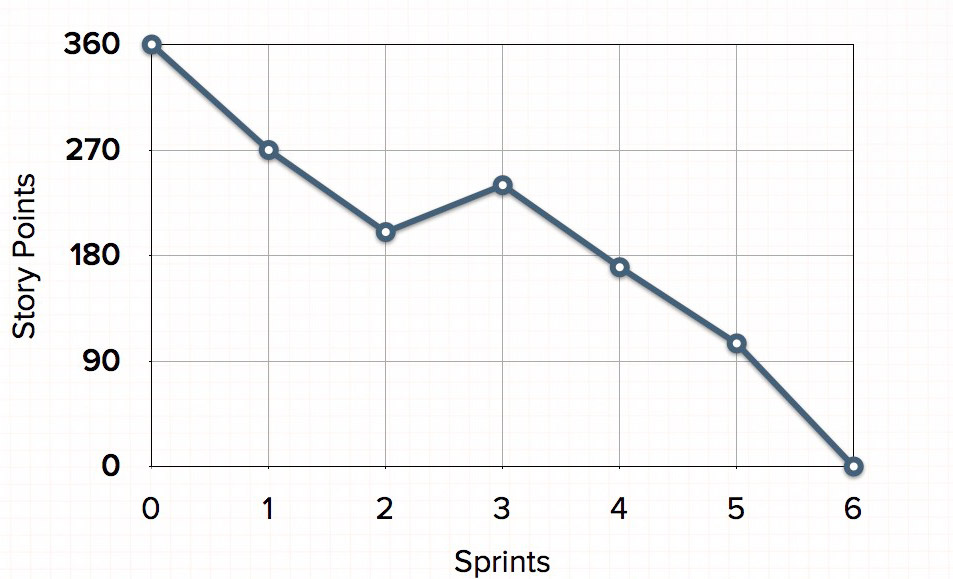
\includegraphics[width=1.0\linewidth]{BDChart.jpg}
	\caption{ An example of a burn down chart \cite{MGS}.}
\end{figure}
	
The figure above shows an example of a burn down chart. This chart is recording the number of story points or user stories left after each sprint. Velocity could have also been used with this graph to make predictions earlier on in the process. 

Difference software will likely need different metrics  \cite{Misra}. %CHECK!
 A simple metric to use in a burn down chart is to record how many user stories are completed in a single sprint. This may work for smaller projects. The issue with this metric is that different user stories may take different amounts of time. Also nearer the end if bugs get put on the backlog this may lead to an invalid velocity.

Using user stories as a metric could be a sufficient way to measure progress in a smaller piece of software. This is because there will be less user stories. In enterprise software most of the user stories will relate to the software again making user stories a more suitable metric. However in games development there will user stories relating graphics, audio and many other parts of the game. 

Downey and Sutherland have a method where points are assigned to a user story. These points can be based on it's size, importance or the time it'll take to complete \cite{Downey}. Then user stories are chosen based on their points, then a baseline velocity for that sprint is calculated from those points. This metric could be suitable for the games industry as it would allow user stories from different parts of the game to be prioritized. ... However an issue with this could be that the importance of of a user story could be subjective. 


There are many reasons for having a metric. Firstly Hartmann says that "measurement drives behaviour" \cite{Hartmann}.  %FIND PAGE!
Selecting a metric can measure progress but can also aid business decisions and may effect team morale. 
Hartmann and Dymond point out that "measurement drives behaviour ". Therefore the metrics can de designed to shape the software development process.....   Also different types of development, enterprise software is more cost driven, game development is more about quality or lack of bugs. 


The software development process will change for different software, for example a large piece of enterprise software the process differ from the process behind making a game. Metrics such as burn down charts would be effective for business software as ....

% TODO:
% Fix focus on question a bit more
% Use a couple more references
% More analysis

%Misra - invent the metric as you need it
%	Selecting a metric because it is commonly used may not give useful data
%	- breaks it down to 4 metric types

%Paper 5 looks at designing agile metrics


\section{Conclusion}
In conclusion ... % dif software/game etc needs dif metric	
	
\bibliographystyle{ieeetr}
\bibliography{comp150_agile}
	
\end{document}
